%% LyX 2.3.2 created this file.  For more info, see http://www.lyx.org/.
%% Do not edit unless you really know what you are doing.
\documentclass[english]{beamer}
\usepackage{lmodern}
\renewcommand{\sfdefault}{lmss}
\renewcommand{\ttdefault}{lmtt}
\usepackage[T1]{fontenc}
\usepackage[latin9]{inputenc}
\setlength{\parskip}{\medskipamount}
\setlength{\parindent}{0pt}
\usepackage{amsmath}
\usepackage{amssymb}
\usepackage{graphicx}
\usepackage{amsmath,amssymb}

\makeatletter

%%%%%%%%%%%%%%%%%%%%%%%%%%%%%% LyX specific LaTeX commands.
\pdfpageheight\paperheight
\pdfpagewidth\paperwidth


%%%%%%%%%%%%%%%%%%%%%%%%%%%%%% Textclass specific LaTeX commands.
% this default might be overridden by plain title style
\newcommand\makebeamertitle{\frame{\maketitle}}%
% (ERT) argument for the TOC
\AtBeginDocument{%
  \let\origtableofcontents=\tableofcontents
  \def\tableofcontents{\@ifnextchar[{\origtableofcontents}{\gobbletableofcontents}}
  \def\gobbletableofcontents#1{\origtableofcontents}
}

%%%%%%%%%%%%%%%%%%%%%%%%%%%%%% User specified LaTeX commands.
\usetheme{Madrid}
\hypersetup{pdfpagemode=None}
\usepackage{tikz}
\usetikzlibrary{shapes.multipart}
\usetikzlibrary{decorations.pathreplacing}
\AtBeginSection[]
{
  \begin{frame}
    \frametitle{Table of Contents}
    \tableofcontents[currentsection]
  \end{frame}
}

\makeatother

\usepackage{babel}
\begin{document}
\title[Spectral properties of the graph Laplacian]{Spectral properties of the graph Laplacian matrix on a 2-sphere}
\author{Martino Milani}
\institute[EPFL - PoliMi]{Department of Mathematics \\EPFL - Politecnico di Milano}
\makebeamertitle

\section*{Outlines}

\beamersetuncovermixins{\opaqueness<1->{45}}{\opaqueness<1->{95}}
\begin{frame}{Outline of the Talk}

\tableofcontents{}
\end{frame}

\section{Introduction}
\begin{frame}[<+>]{The problem}

\begin{block}{Problem}
Design an algorithm to filter (convolve) discrete signals on the
2-sphere
\end{block}
\begin{itemize}
\item Computationally efficient
\item Easy to be learned in a CNN
\item We want the filtering operation to be equivariant to rotations $SO(3)$
\end{itemize}
\end{frame}
%
\begin{frame}{The solution}

\begin{block}{Problem}
Design an algorithm to filter discrete signals on the 2-sphere
\end{block}
%
\begin{block}{Solution}
Filtering with a polynomial of the graph Laplacian matrix $\mathbf{L}$
\begin{equation}
F(\mathbf{f})=P_{K}(\mathbf{L})\mathbf{f}=\sum_{k=0}^{K}\theta_{k}\mathbf{L}^{k}\mathbf{f}
\end{equation}
\end{block}
\begin{itemize}
\item Computationally efficient since the graph is sparse, thus $\mathbf{L}^k$
is sparse
\item Filter defined with $K$ parameters: the coefficients $\theta_{k}$
of the polynomial $P_{K}(\mathbf{L})$
\item \textbf{Is this filtering equivariant to rotations $SO(3)$?}
\end{itemize}
\end{frame}
%
\begin{frame}{\textbf{Is this filtering }$F(\mathbf{f})=P_{K}(\mathbf{L})\mathbf{f}=\sum_{k=0}^{K}\theta_{k}\mathbf{L}^{k}\mathbf{f}$\textbf{
equivariant to rotations $SO(3)$?}}
\begin{block}{Answer:}
 Yes, if the eigenspaces of $\mathbf{L}$ and $\triangle$ are ``the
same''.
\end{block}
\begin{itemize}
\item Remark: $\mathbf{L}$ is a matrix and $\triangle$ is a continuous operator. This convergence is rigorously stated in \cite{vonluxburg2008} 
\item Two roads:
\begin{itemize}
\item We could aim at building $\mathbf{L}$ such that $\mathbf{Eig}\mathbf{L}\xrightarrow{N\to\infty}\mathbf{Eig}\mathbf{\triangle}$ (common approach in literature) \cite{NIPS2006_2989}
\item Alternatively, we could aim at building $\mathbf{L}$ such that $\mathbf{Eig}\mathbf{L}=\mathbf{Eig}\mathbf{\triangle}$
up to a certain bandwidth. We tried, we failed.
\end{itemize}
\end{itemize}
\end{frame}
%

\section{Existing results}
\begin{frame}{Existing convergence results: random sampling on any compact manifold}

Results exist for a \textbf{random }sampling and for \textbf{any compact
infinitely differentiable Riemannian submanifold of $\mathbb{R}^{N}$
}where the adjacency matrix is defined as follows 
\begin{equation}
W_{ij}=e^{\frac{||x_{i}-x_{j}||^{2}}{4t}}
\end{equation}
 bringing to the following definition

\begin{definition}{Heat kernel graph Laplacian operator} 	$$L_n^t:\quad(L_n^tf)(y) = \frac{(4\pi t)^{-\frac{k+2}{2}}}{n}\left(f(y)\sum_i e^\frac{||x_i-y||}{4t}-\sum_ie^\frac{||x_i-y||}{4t}f(x_i)\right)$$ \label{def:heatkernelgraphlaplacian}\end{definition}
\end{frame}
%
\begin{frame}{Existing convergence results: random sampling on any compact manifold}

From \cite[Belkin et al, "Convergence of Laplacian Eigenmaps"]{NIPS2006_2989}

 \begin{theorem}  \label{theo:convergence}	Let $\lambda_{n,i}^t$ be the ith eigenvalue of $L_n^t$ and $e^t_{n,i}$ be the corresponding eigenfunction (which for each fixed i will be shown to exist for t sufficiently small). Let $\lambda_{i}$ be the ith eigenvalue of $\triangle_\mathcal M$ and $e_{i}$ be the corresponding eigenfunction. Then there exists a sequence $t_n\rightarrow 0$ such that  	  	$$\lim_{n\rightarrow\infty} \lambda_{n,i}^{t_n}=\lambda_i$$  	$$\lim_{n\rightarrow\infty}||e_{n,i}^{t_n}(x) - e_i(x)||_2 = 0$$  	  	where the limits are in probability.  	  \end{theorem}
\end{frame}
%
\begin{frame}{DeepSphere1.0 \cite[Deferrard et al]{DBLP:journals/corr/abs-1810-12186}: we don't
see the expected convergence!}

Differences between the setting of the previous theorem:
\begin{itemize}
\item Not random sampling, but deterministic - \textbf{HEALPix} -
\item Not a full graph, but fixed number of neighbors
\end{itemize}

\begin{figure}
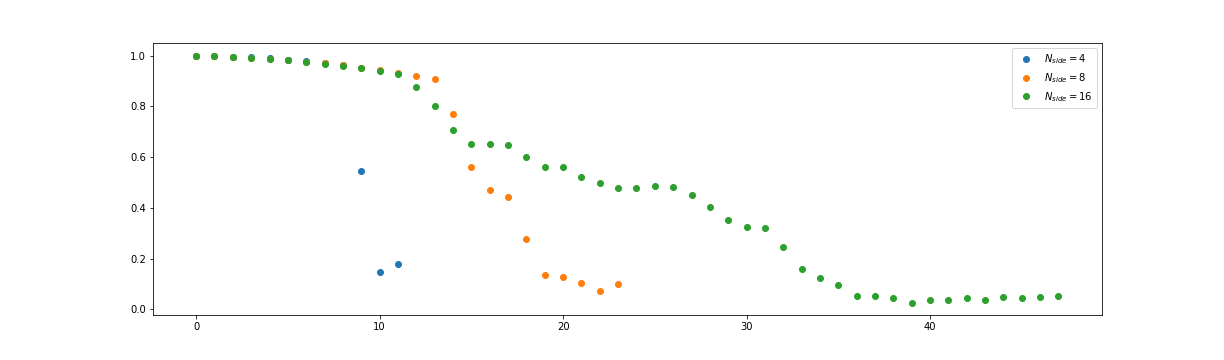
\includegraphics[scale=0.15]{/Users/Mart/Documents/EPFL/PDM/codes/05_figs/old_results2}

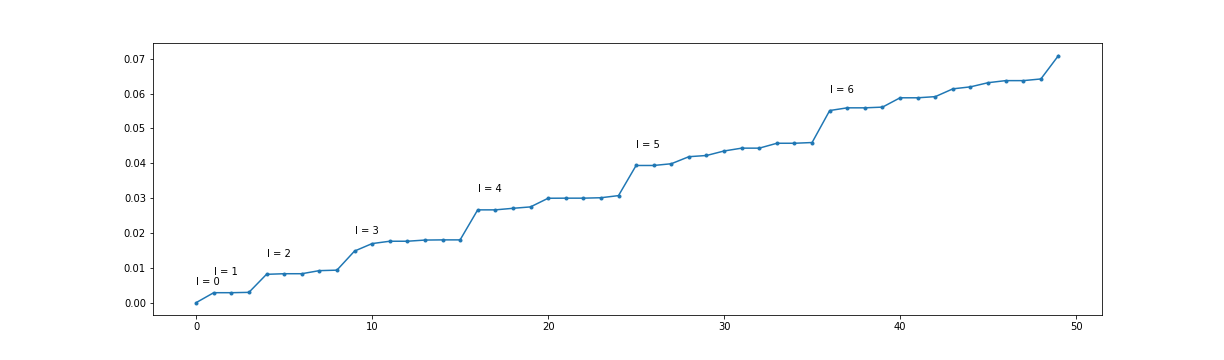
\includegraphics[scale=0.15]{/Users/Mart/Documents/EPFL/PDM/codes/05_figs/old_results3}\caption{Above: alignment of the eigenspaces of $\mathbf{L}$ and $\triangle$.
Under: eigenvalues of the graph Laplacian matrix for $N_{side}=16$
in DeepSphere architecture, from \cite{DBLP:journals/corr/abs-1810-12186}}

\end{figure}
\end{frame}
%

\section{New results}
\begin{frame}{DeepSphere2.0}

Differences between the setting of DeepSphere1.0 \cite{DBLP:journals/corr/abs-1810-12186}:
\begin{itemize}
\item \textbf{Number of neighbors increasing with $N_{side}$}
\item Slightly modified kernel width $t$ in definition \ref{def:heatkernelgraphlaplacian}
\end{itemize}

\begin{figure}
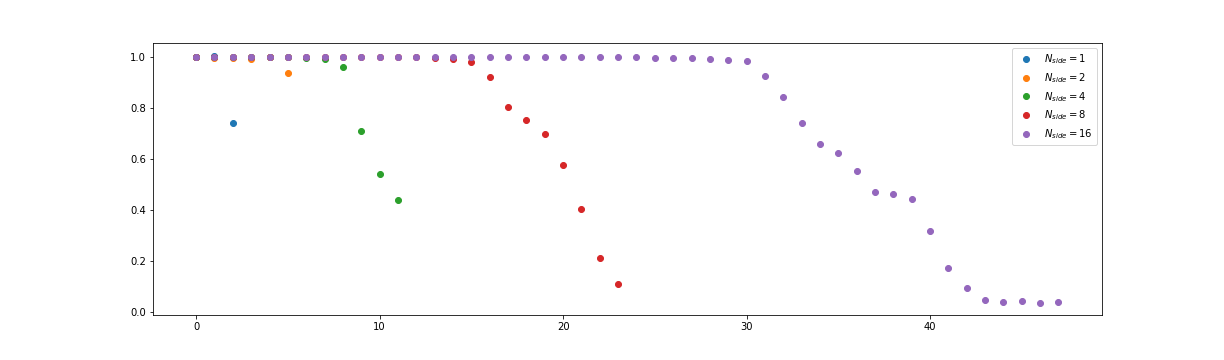
\includegraphics[scale=0.15]{/Users/Mart/Documents/EPFL/PDM/codes/06_figures/optimal_thresholded_diagonal}

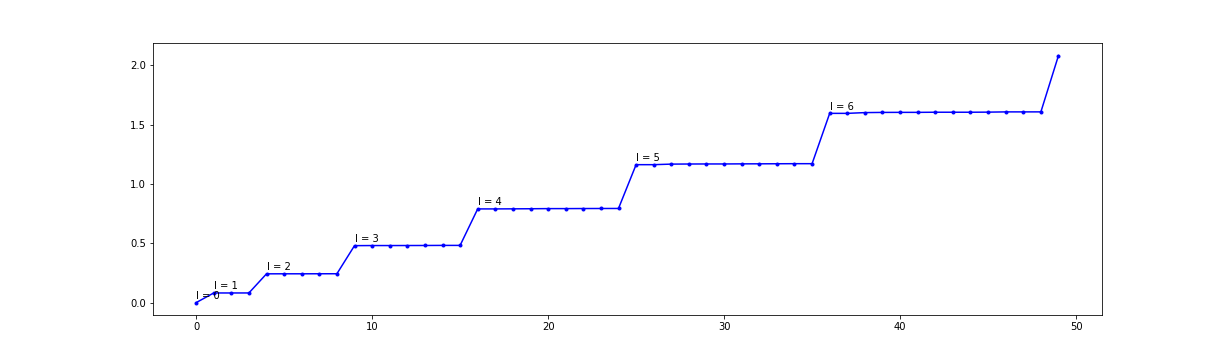
\includegraphics[scale=0.15]{/Users/Mart/Documents/EPFL/PDM/codes/06_figures/optimal_thresholded_eigenvalues}\caption{Above: alignment of the eigenspaces of $\mathbf{L}$ and $\triangle$.
Under: eigenvalues of the graph Laplacian matrix for $N_{side}=16$
in the new architecture}
\end{figure}

\end{frame}
%

\section{Current and future work}
\begin{frame}{Current research questions}
\begin{itemize}
\item We observed the experimental convergence. Can we quantify it, using
the fact that we know we are on a sphere?
\item So far we used a graph to build the sparse matrix $\mathbf{L}$ that
approximates the Laplace-Beltrami operator $\triangle$. However,
there are different ways of building a matrix that approximates a
continuous operator, one of them being the \textbf{Finite Element
Method.}
\end{itemize}
\end{frame}
%
\begin{frame}{Alternatives to the heat kernel graph Laplacian: FEM Laplacian}

In \cite[Discrete Laplace Beltrami operators for shape analysis and segmentation]{REUTER2009381}
the Cubic FEM Laplacian on a sphere shows a spectrum that is much
closer to the spherical harmonics than the one of the used in \cite{DBLP:journals/corr/abs-1810-12186}.

\begin{figure}

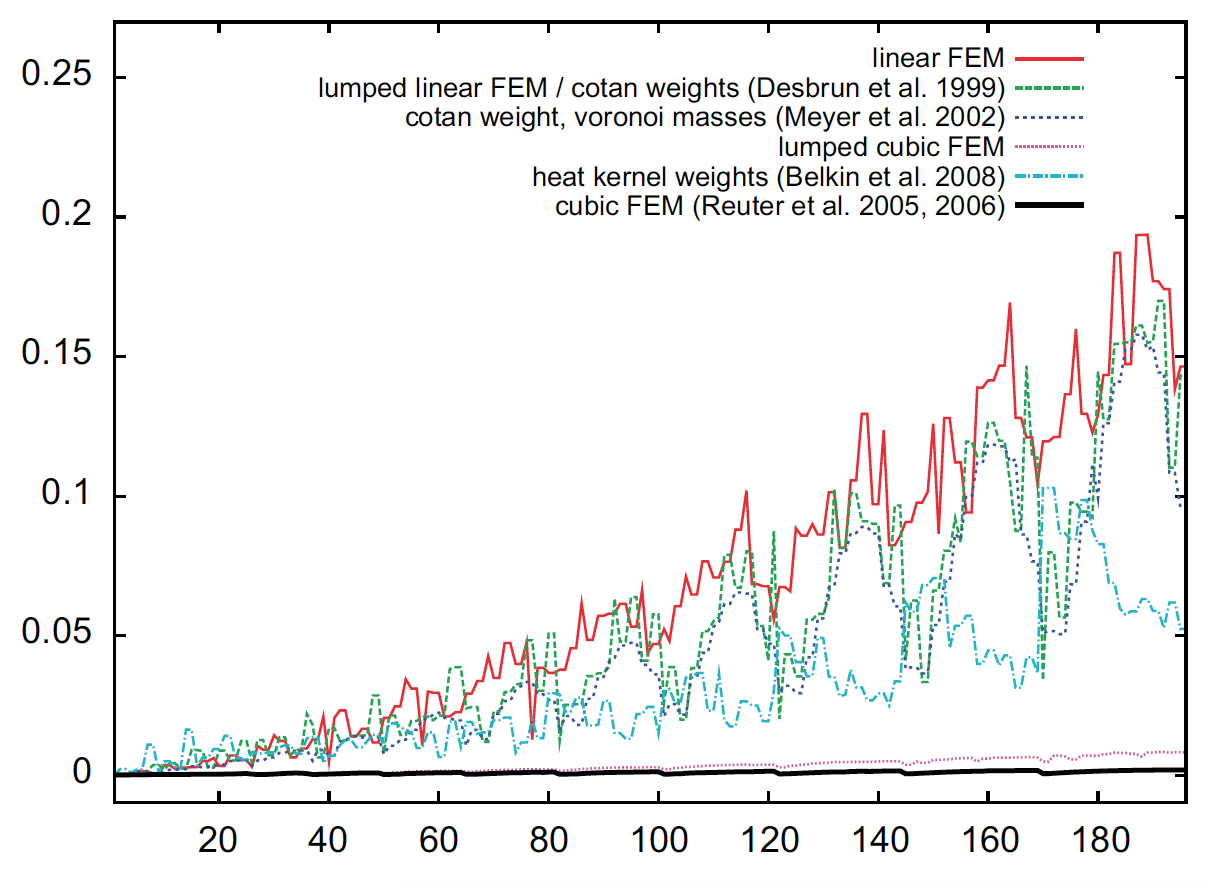
\includegraphics[width=0.45\paperwidth]{eigenfunctions}\caption{Error of eigenfunctions on the sphere, from \cite{REUTER2009381}}

\end{figure}
\end{frame}
%
\begin{frame}{FEM approximation of the Laplace-Beltrami operator}
\begin{block}{The eigenvalue problem}
The weak form of the eigenvalue problem solved in a finite element
space $V_{h}$ is the following
\begin{equation}
(\triangle f_{h},\phi_{h})_{L^{2}(\mathcal{S})}=\lambda(f_{h},\phi_{h})_{L^{2}(\mathcal{S})}\quad\forall\phi_{h}\in V_{h}
\end{equation}
\end{block}

It is equivalent to the generalized eigenvalue problem
\begin{equation}
L\mathbf{f}=\lambda B\mathbf{f}
\end{equation}

where $L$ is the semi positive definite stiffness matrix $(L)_{ij}=(\triangle\phi_{i},\phi_{j})_{L^{2}(\mathcal{S})}$
and $B$ is the positive definite mass matrix $(B)_{ij}=(\phi_{i},\phi_{j})_{L^{2}(\mathcal{S})}$.

Observe that to compute $L$ and $B$ we need to compute integrals
over some triangulation of the manifold, so this method is inherently
different from computing the graph Laplacian!

\end{frame}
%
\begin{frame}{FEM approximation of the Laplace-Beltrami operator}

For the FEM method, we know the order of convergence of the spectrum
of $L$ (we don't have it for the Graph Laplacian). Plus, we know
experimentally from \cite{REUTER2009381} that the FEM discretization
has a better spectrum.
\begin{block}{Convergence results (from \cite{REUTER2009381})}
With mesh size $h$ and order $p$ functions the eigenvalues converge
with order $2p$ and the eigenfunctions with order $p+1$ in the $L_{2}$
norm, as long as the geometry is correctly represented.
\end{block}
\end{frame}
%
\begin{frame}{FEM Laplacian VS heat kernel graph Laplacian}

\begin{block}{Heat kernel graph Laplacian}
\[
(L)_{ij}= \begin{cases}
 \sum_{k}e^{-\frac{||x_{i}-x_{k}||^{2}}{4t}} &i=j\\
  -e^{-\frac{||x_{i}-x_{j}||^{2}}{4t}} & i\neq j
\end{cases}  
\]
\scriptsize{
\begin{itemize}
\itemsep0em 
\item Easily sparsified by thresholding the weights
\item Even if sparsified, it still shows the expected convergence proved
in \cite{NIPS2006_2989}
\item Easy to incorporate the information that we know the manifold by using the geodesic distance instead of the euclidean distance
\end{itemize}}
\end{block}

\begin{block}{FEM Laplacian}

\[
(L)_{ij}=   \int_{\mathcal{S}}\triangle_\Gamma\phi_{i}\phi_{j}
\]
\scriptsize{\begin{itemize}
\itemsep0em 
\item Easily sparsified by the choice of the basis functions $\{\phi_{i}\}$
\item Strong convergence results: theorem \ref{theo:convergence} (convergence
rate for the spectrum)
\item hard to incorporate the information that we know the manifold
\end{itemize}}
\end{block}
%
\end{frame}
\section{Conclusions}
\begin{frame}{Conclusions}
\begin{itemize}
	\item We got a much better understanding of the spectral properties of the heat kernel graph Laplacian and their dependencies on two key parameters: the kernel width and the number of neighbors. 
	\item We successfully improved the spectral properties of the heat kernel graph Laplacian used in DeepSphere \cite{DBLP:journals/corr/abs-1810-12186}. Next step is trying to quantify the error theoretically.
	\item New exciting direction: from a Graph-CNN, to a FEM-CNN?
\end{itemize}


\end{frame}
%


\section{Appendix}

\begin{frame}{Kernel width}
\begin{figure}
	
	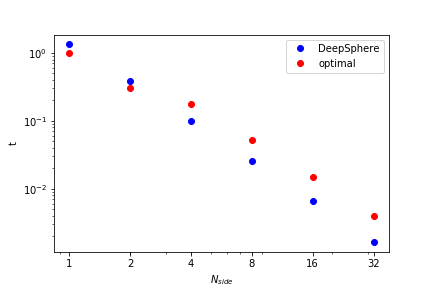
\includegraphics[width=0.6\paperwidth]{kernelwidth}\caption{Kernel width $t$}
	
\end{figure}
\end{frame}
\begin{frame}{Kernel width: DeepSphere VS "optimal"}
\begin{figure}
	\centering
	
	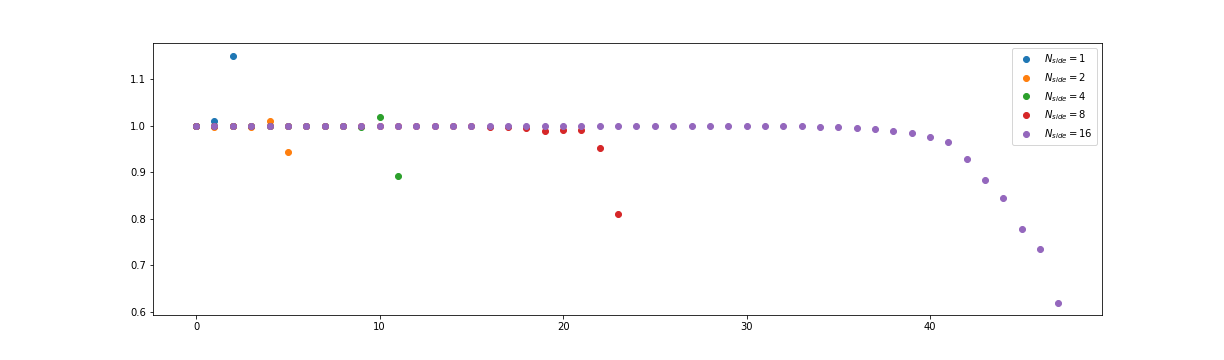
\includegraphics[width=0.8\paperwidth]{optimal_full_diagonal}
	
	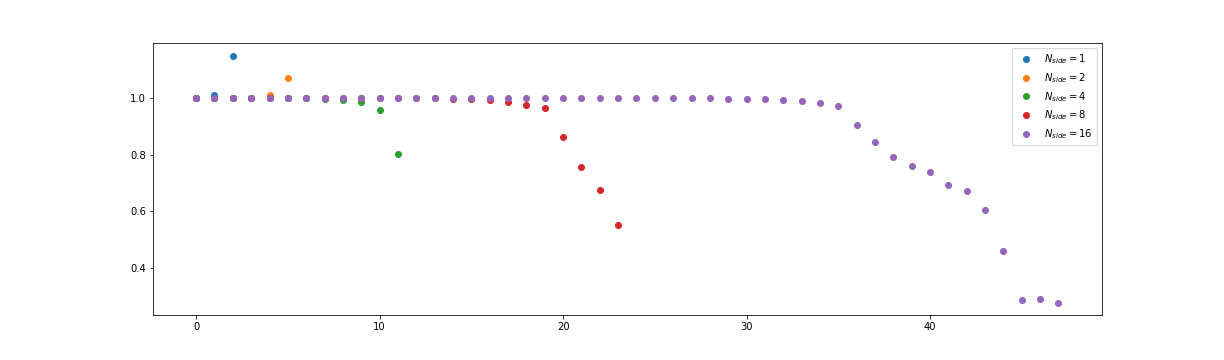
\includegraphics[width=0.8\paperwidth]{deepsphere_full_diagonal}
	
	\caption{On top, full optimal graph. At the bottom, full DeepSphere graph}
\end{figure}

\end{frame}
\begin{frame}{DeepSphere: sparsity analysis}
\begin{figure}
	\centering
	
		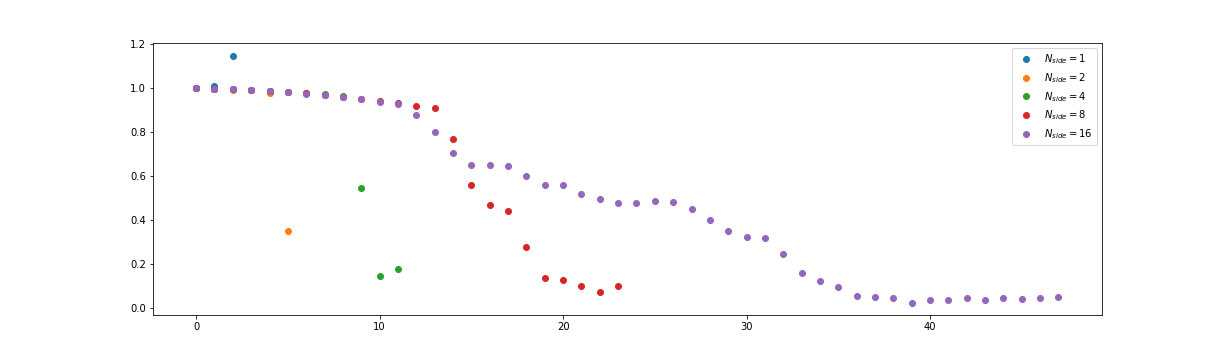
\includegraphics[height=0.8in]{deepsphere_original_diagonal}
		
		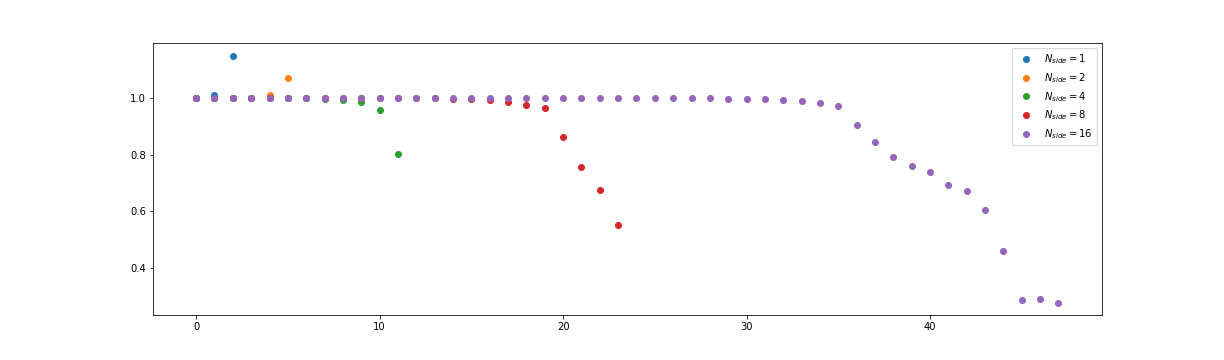
\includegraphics[height=0.8in]{deepsphere_full_diagonal}
	
	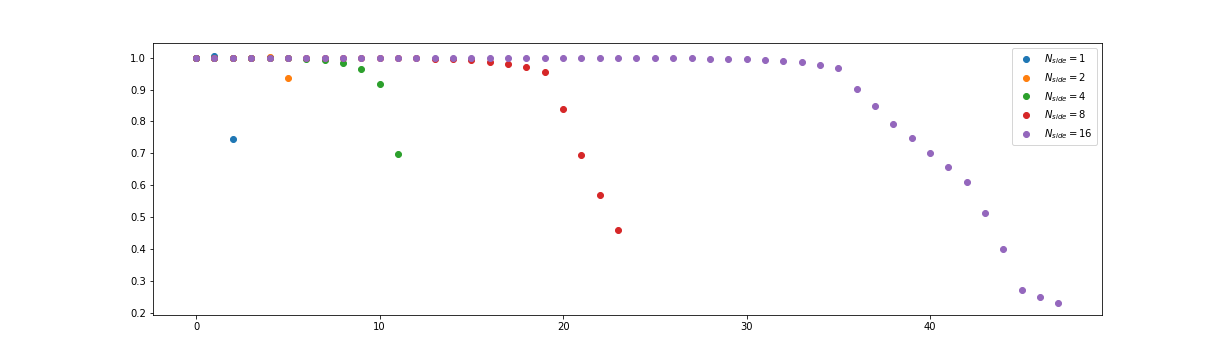
\includegraphics[height=0.8in]{deepsphere_thresholded_diagonal}
	

	\caption{\scriptsize{On top, DeepSphere original graph (fixed number of neighbors). In the middle, DeepSphere full graph. At the bottom, DeephSphere graph thresholded at 0.01 (increasing number of neighbors)}}
\end{figure}

\end{frame}

\begin{frame}{$t$ sensitivity}
\begin{figure}
	
	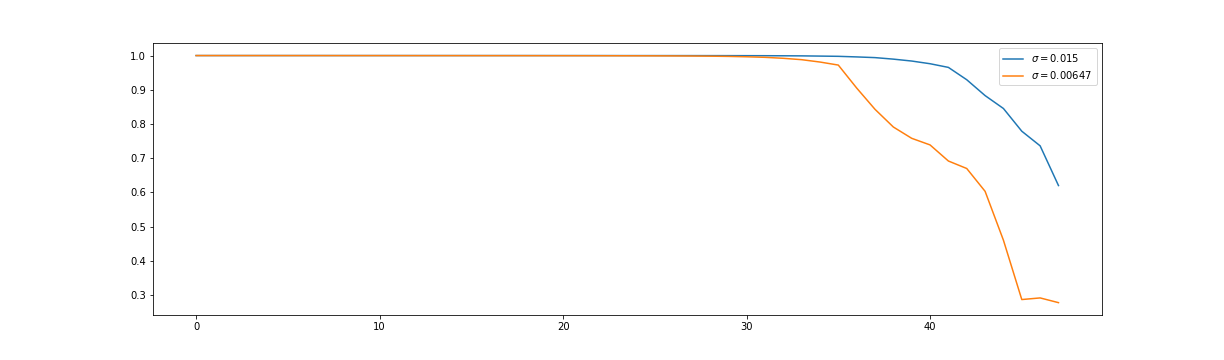
\includegraphics[width=0.8\paperwidth]{t_sensitivity_diagonal}\caption{The spectrum is highly sensible to little changes of the kernel width}
	
\end{figure}
\end{frame}

\begin{frame}[allowframebreaks]{Bibliography}

\bibliographystyle{plain}
{\small {\bibliography{/Users/Mart/Documents/EPFL/PDM/report/references}}}
\end{frame}


\end{document}
